% AASTeX v6.2
%\documentclass[preprint]{aastex62}

% ApJ Format
\documentclass[iop,revtex4,twocolumn,apj,numberedappendix,appendixfloats]{emulateapj}
\usepackage{apjfonts}
% Hyperlinks & Bookmarks
\usepackage[pagebackref=false,colorlinks=true,citecolor=blue,linkcolor=blue,breaklinks=true,bookmarks=true]{hyperref}
\usepackage{amsmath}
\usepackage{comment}

% Units
\newcommand{\kms}{km~s$^{-1}$}
\newcommand{\msun}{$M_{\odot}$}
\newcommand{\msunyr}{$M_{\odot}~{\rm yr}^{-1}$}
\newcommand{\lsun}{$L_{\odot}$}
\newcommand{\ergs}{erg~s$^{-1}$}
\newcommand{\cmsq}{cm$^{-2}$}
\newcommand{\um}{$\mu$m}
\newcommand{\uJy}{$\mu$Jy}
\newcommand{\sqdeg}{deg$^2$}
\newcommand{\lx}{$L_{\rm X}$}
\newcommand{\lmir}{$L_{\rm 12\mu m}$}
\newcommand{\loiii}{$L_{\rm [OIII]}$}
% Emission lines
\newcommand{\Ha}{H$\alpha$}
\newcommand{\Hb}{H$\beta$}
\newcommand{\OII}{[O\,{\sc ii}]}
\newcommand{\OIIlam}{[O\,{\sc ii}]\,$\lambda$3727}
\newcommand{\SII}{[S\,{\sc ii}]}
\newcommand{\OIII}{[O\,{\sc iii}]}
\newcommand{\OIIIlam}{[O\,{\sc iii}]\,$\lambda$5007}
\newcommand{\NII}{[N\,{\sc ii}]}
\newcommand{\NeIII}{[Ne\,{\sc iii}]}
% special 
\newcommand{\nod}{\nodata}

\newcommand{\angstrom}{\mbox{\normalfont\AA}}
\newcommand{\reff}{$R_{\rm eff}$}
\newcommand{\ewha}{EW(H$\alpha$)}
\newcommand{\logm}{log({\it M}/M$_{\odot}$)}
%\newcommand{\arcsec}{\prime\prime}

% citations
\defcitealias{Fu18}{Paper I} 

\usepackage{epstopdf}

\begin{document}

\title{SDSS-IV MaNGA: Radial Profiles of Specific Star Formation Rate in Nearby Interacting Galaxies}

\author{
Joshua L. Steffen\altaffilmark{1}, 
Hai Fu\altaffilmark{1}, and 
MaNGA Team 
}
\altaffiltext{1}{Department of Physics \& Astronomy, The University of Iowa, 203 Van Allen Hall, Iowa City, IA 52242}

\begin{abstract}
We study the spatial profile of the star formation rate (SFR) in a sample of XXX interacting galaxies within the MaNGA (Mapping Nearby Galaxies at Apache Point Observatory) survey. We find that the specific star formation rate (sSFR) is centrally enhanced in the centers of the interacting galaxies by $\sim$XXX and in their disks by $\sim$XXX. We further investigate how these profiles behave as a function of stellar mass, mass ratio, and projected separation. We find that the sSFR profiles are unaffected by the stellar masses of the interacting galaxies; however, they are affected by the mass ratio between the galaxies where the galaxies with the smallest mass ratio feature the largest enhancement. We also find that, in pairs with large mass ratios (XX$-$XX), the less massive galaxy of the pair has slightly higher levels of sSFR enhancement, $\sim$0.1 dex. We also find that the level of sSFR enhancement increases with closer projected separations; however, the closest pairs, $\le$5 kpc, show no signs of sSFR enhancement/suppression. We suspect that these close pairs are merging galaxies which have passed their first pericenter, but haven't had enough time pass for the merger-induced gas inflows to trigger new star formation. We also set a simple model for the future mass growth of the interacting galaxies due to the merger-induced star formation. We predict that the paired galaxies in our sample will see a mass growth rate which is XX$\times$ higher than secular mass growth. 
\end{abstract}

\keywords{galaxies: active --- galaxies: nuclei --- galaxies: interactions}

%%%%%%%%%%%%%%%%%%%%%%%%%%%%%%%%%%%%%%%%%%%%%%%%%%%%
\section{Introduction}\label{sec:intro}

%%%Galaxy Evolution%%%
In the $\Lambda$CDM model, galaxy evolution is a hierarchical process. Over the lifetime of the universe, smaller galaxies have iteratively merged with each other to form more massive galaxies. In fact, cosmological hydrodynamical simulations have shown that repeated merger events may be responsible for as much as $\sim$60\% of stellar mass in massive galaxies like M87 (e.g. \citet{Rodriguez-Gomez:2016}; \citet{Pillepich:2018}). 

%%%Simulations%%%
The internal dynamics of these interacting galaxies were first modeled in the seminal work, \citet{Toomre:1972}. Since then, hydrodynamical simulations have expanded upon the N-body simulations of \citet{Toomre:1972} by modeling gas-dynamics within the galaxies. These simulations show how barred structures develop within the disks of the interacting galaxies due to the tidal torques between them \citep{Barnes:1991}. As the bars form, the gases within the galaxy's disk lose angular momentum and get funneled into the centers of the galaxies. 

When the gas-inflows impact upon the gases in the nucleus of galaxy a burst of new star formation in triggered \citep{Barnes:1996, Mihos:1996}. These gas inflows will also bring metal-poor gases from the disk into the center of the galaxy which can dilute the central metallicity \citep{Rupke:2010, Perez:2011, Scudder:2012}. The gas-inflows may also be able to make it into very center of the galaxy and trigger supermassive black hole (SMBH) accretion \citep{Capelo:2017}. 

%%%Observations%%%
Centrally enhanced star formation has also been observed in large spectroscopic surveys including; CfA2  \citep{Barton:2000, Woods:2006}, 2dF \citep{Lambas:2003}, AEGIS \citep{Lin:2007}, SDSS \citep{Ellison:2008}, COSMOS \citep{Kartaltepe:2007,Xu:2012}, PRIMUS \citep{Wong:2011}, and GAMA \citep{Robotham:2014}.

This star formation enhancement increases with closer projected separations between the two galaxies \citep{Ellison:2008, Scudder:2012} but has still shown to be detectable at wide projected separations of 150 kpc \citep{Patton:2013}. The level of the star formation enhancement also increases with smaller stellar mass ratios, $|\Delta log {\it M} |$, between the two galaxies \citep{Ellison:2008}. 

%%%Integral Field Spectroscopy%%%
With the recent large integral field spectroscopic (IFS) surveys, interacting galaxies can be studied in unprecedented spatial detail. Where previous spectroscopic surveys were limited to the nucleus of the interacting galaxies, the new IFS surveys will be able to study both the nuclei and the disks of the interacting galaxies. 

The IFS surveys, CALIFA\footnote{Calar Alto Legacy Integral Field Area} and MaNGA\footnote{Mapping Nearby Galaxies at Apache Point Observatory}, have already been used to study the SFR of interacting galaxies in merging galaxies. The SFR was found to be centrally enhanced by a factor of 2$-$3$\times$ \citep{Barrera-Ballesteros:2015, Pan:2019}, which is in agreement with previous single-fiber spectroscopic surveys. These surveys also studied the SFR in the disk of the paired galaxies; however, there is a discrepancy between the results. \citet{Barrera-Ballesteros:2015} found a suppression to the SFR of $\sim$0.74$\times$ while \citet{Pan:2019} found an enhancement of 1.22$-$1.58$\times$. 

{\it can I mention Barrera-Ballesteros+15 and Pan+19 together like this since the BB uses ewha as a proxy for SFR and Pan uses sSFR?}

The MaNGA survey has also been used to study the radial profiles of SFR in post merger galaxies, which are the galaxies which have recently coalesced. The post merger galaxies showed a central enhancement to the SFR surface density of 2.5$\times$ and an enhancement in their disks of 1.26$\times$ \citep{Thorp:2019}.

%%%Purpose%%%
In our previous work, \citet{Fu:2018}, we built a sample of paired galaxies in the MaNGA survey where both components of the pair were contained within field of view of a single IFU. We found that approximately 5.7\% of the MaNGA galaxies have a companion galaxies contained with the IFU. In this work, we will use a version of this sample updated for the recent MaNGA Data Release 16 (DR16) and further supplement this with a sample of companion galaxies identified outside the field of view of the IFUs. 

In this work we will expand upon the previous works by studying how the spatial profile of SFR behaves as a function of the stellar mass of the paired galaxy, the mass ratio between the galaxy pairs, and the projected separation between the galaxies. We will also model how the merger-induced star formation will affect the future mass growth of the interacting galaxies. 

% Organization
This paper is organized as follows; in Section \ref{sec:data} we will discuss the detail of the MaNGA survey, in Section \ref{sec:analysis} we will discuss how we extract emission lines from the MaNGA survey and how we calculate the star formation from them, in Section \ref{sec:pair} we discuss the construction of our pair sample, in Section \ref{sec:control} we discuss the construction of our control sample, in Section \ref{sec:radial} we build the radial profiles for the pair and control galaxies, in Section \ref{sec:results} we discuss the results of the survey, in Section \ref{sec:discussion} we discuss our results in the context of other surveys, and in Section \ref{sec:sum} we summarize and conclude the work. 

%%%%%%%%%%%%%%%%%%%%%%%%%%%%%%%%%%%%%%%%%%%%%%%%%%%%
\section{Data}\label{sec:data}

MaNGA is an a IFS survey based at Apache Point Observatory (APO) which used the SDSS 2.5 meter telescope along with two dual-channel BOSS spectrographs. MaNGA captures spectra through 17 integral field units (IFUs) with variable numbers of fibers; 19, 37, 61, 91, and 127 fibers covering 12.5\arcsec, 17.5\arcsec, 22.5\arcsec, 27.5\arcsec, and 32.5\arcsec on the sky respectively. MaNGA is an optical survey with a spectral coverage of 3600$-$10,300 \AA with a resolution of R $\sim$ 2000 and a median spectra coverage of 2.5\arcsec FWHM \citep{Bundy:2015}. 

MaNGA targets galaxies from a subset of 41,154 galaxies with from the NASA-Sloan Atlas (NSA) with a redshift range of 0.01 $<$ z $<$ 0.15 and a luminosity range of -17.7 $<$ $\mathcal{M_{\rm i}}$ $<$ -24.0, where $\mathcal{M_{\rm i}}$ is the rest frame i-band magnitude within the NSA survey's elliptical Petrosian apertures. MaNGA plans to cover 10,000 galaxies with a flat stellar mass distribution at two spatial coverages, 1.5 \reff\ and 2.5 \reff\ (where \reff\ is the radius which contains 50\% of the galaxy's total light). In this work we use the data from the internal data release, MPL-8, which covers 6142 unique galaxies. 

The MaNGA sample is split into three subsamples; the Primary Sample, Secondary Sample, and Color-Enhanced Sample. The Primary sample contains the galaxies which are covered out to 1.5 \reff\ and makes up 47\% of the survey. The Secondary contains the galaxies which are covered out to 2.5 \reff\ and makes up 37\% of the survey. The Color-Enhanced sample is designed to select rarer galaxy types with a spatial coverage of 2.5 \reff\ and makes up 16\% of the survey. 

Because of the survey's flat stellar mass distribution and uniform spatial coverage, these samples have a unique ``banana" shaped distribution in redshift and luminosity, see Figure \ref{fig:Mi-z}. Because the Secondary and Color-Enhanced samples use a wider spatial coverage than the Primary sample, the Secondary and Color-Enhanced Samples will posses galaxies of higher redshifts than galaxies at the same stellar masses in the Primary sample. 



%%%%%%%%%%%%%%%%%%%%%%%%%%%%%%%%%%%%%%%%%%%%%%%%%%%%
\section{Emission Lines}\label{sec:analysis}


%%%%%%%%%%%%%%%%%%%%%%%%%%%%%%%%%%%%%%%%%%%%%%%%%%%%
\section{Pair Sample}\label{sec:pair}


%%%%%%%%%%%%%%%%%%%%%%%%%%%%%%%%%%%%%%%%%%%%%%%%%%%%
\section{Control Sample}\label{sec:control}


%%%%%%%%%%%%%%%%%%%%%%%%%%%%%%%%%%%%%%%%%%%%%%%%%%%%
\section{Radial Profiles}\label{sec:radial}


%%%%%%%%%%%%%%%%%%%%%%%%%%%%%%%%%%%%%%%%%%%%%%%%%%%%
\section{Results}\label{sec:results}


%%%%%%%%%%%%%%%%%%%%%%%%%%%%%%%%%%%%%%%%%%%%%%%%%%%%
\section{Discussion}\label{sec:discussion}


%%%%%%%%%%%%%%%%%%%%%%%%%%%%%%%%%%%%%%%%%%%%%%%%%%%%
\section{Summary and Conclusion}\label{sec:sum}






\acknowledgments

% funding
J.S. and H.F. acknowledge support from the National Science Foundation (NSF) grant AST-1614326 and University of Iowa funds. 

%%%%%%%%%%%%%%%%%%%% REFERENCES %%%%%%%%%%%%%%%%%%
\bibliographystyle{aasjournal}
\bibliography{mergerbib}

%%%%%%%%%%%%
% Appendix
%%%%%%%%%%%%

\hbox{}\clearpage

\appendix

\section{Figures}

%%%%%%%%%%%%%%%%%%%%%%%%%%%%%%%%%%%%%%%%%%%%%%
\begin{figure}
\centering
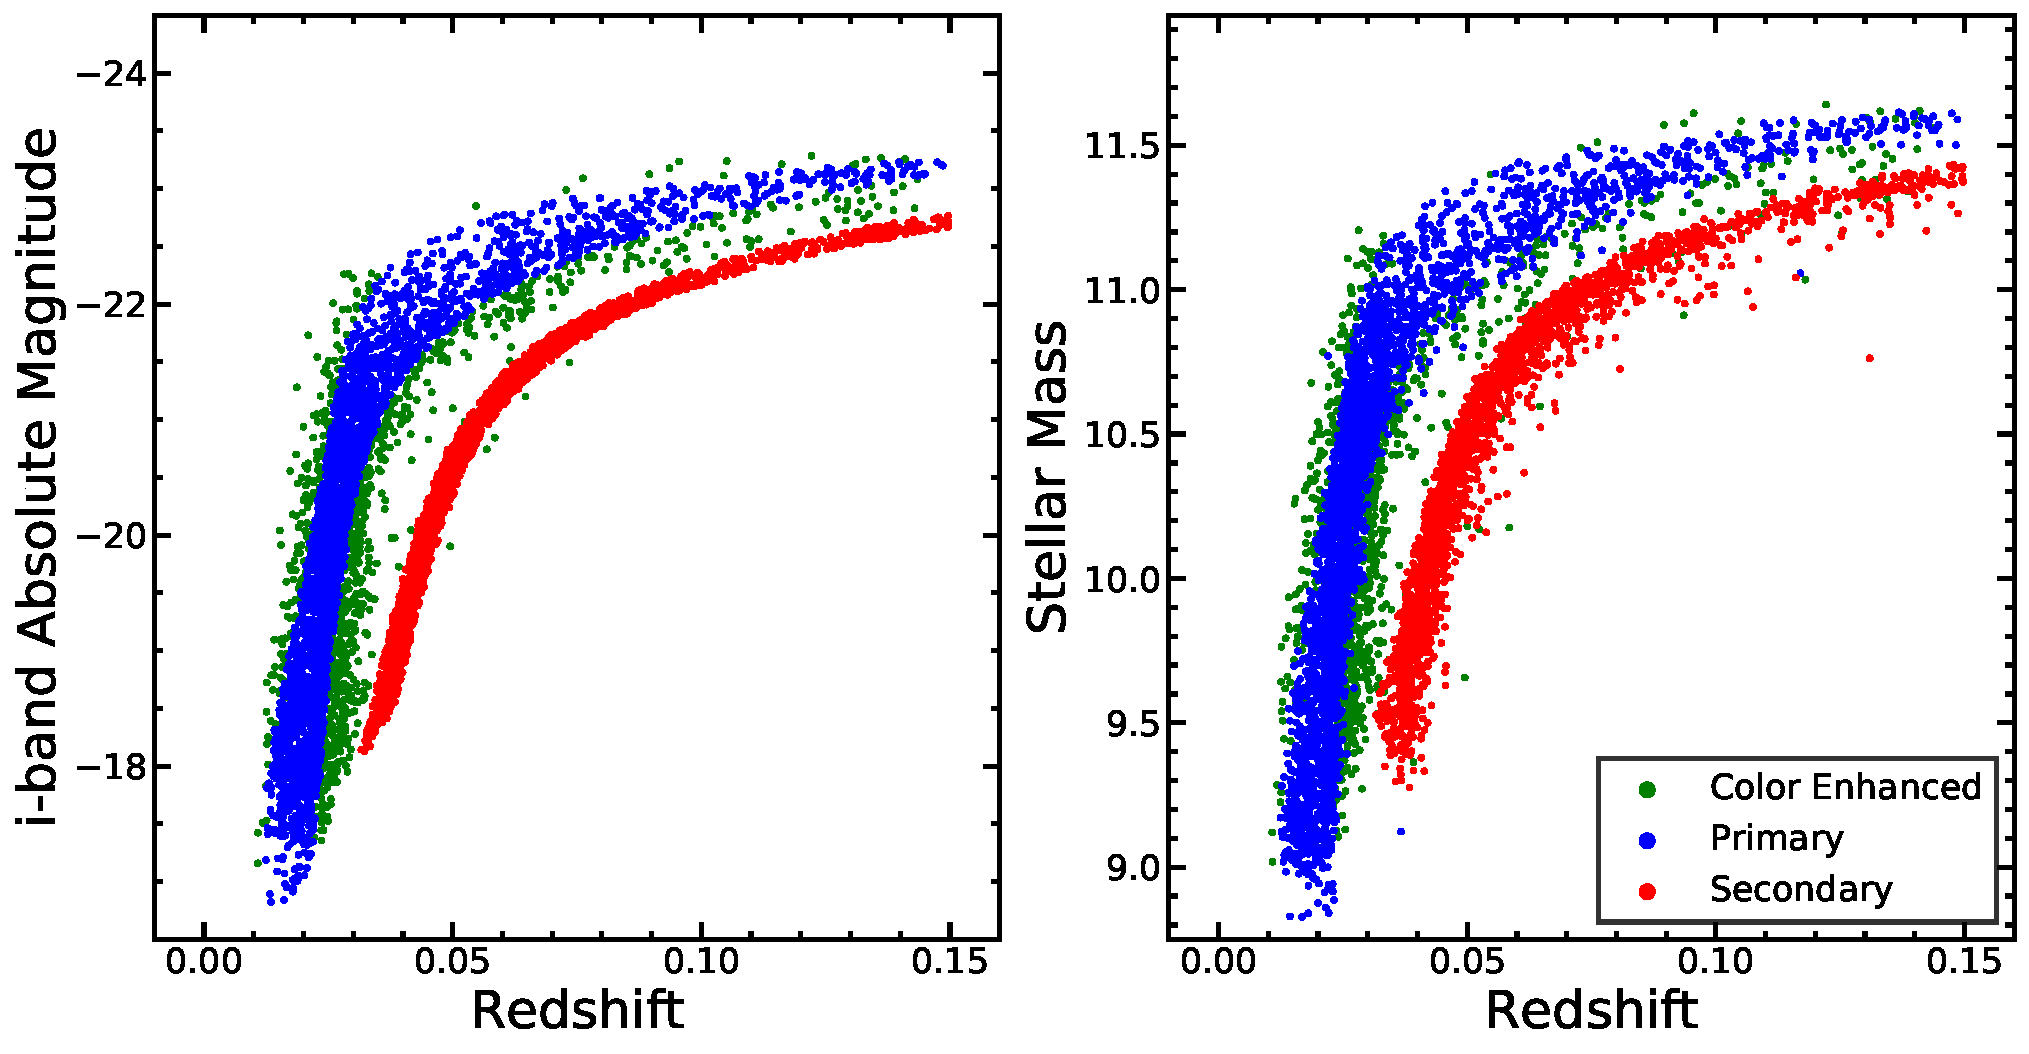
\includegraphics[width=\linewidth]{fig/Mi-z.pdf}
\caption[The luminosity - redshift distribution and mass - redshift distribution of the MaNGA sample.]{On the left is the luminosity - redshift distribution of the MaNGA sample. The figure illustrates the unique distribution of the MaNGA sample. On the right, I replace the luminosity with stellar mass from the NSA catalog.}
\label{fig:Mi-z}
\end{figure}
%%%%%%%%%%%%%%%%%%%%%%%%%%%%%%%%%%%%%%%%%%%%%%

%%%%%%%%%%%%%%%%%%%%%%%%%%%%%%%%%%%%%%%%%%%%%%
\begin{figure}
\centering
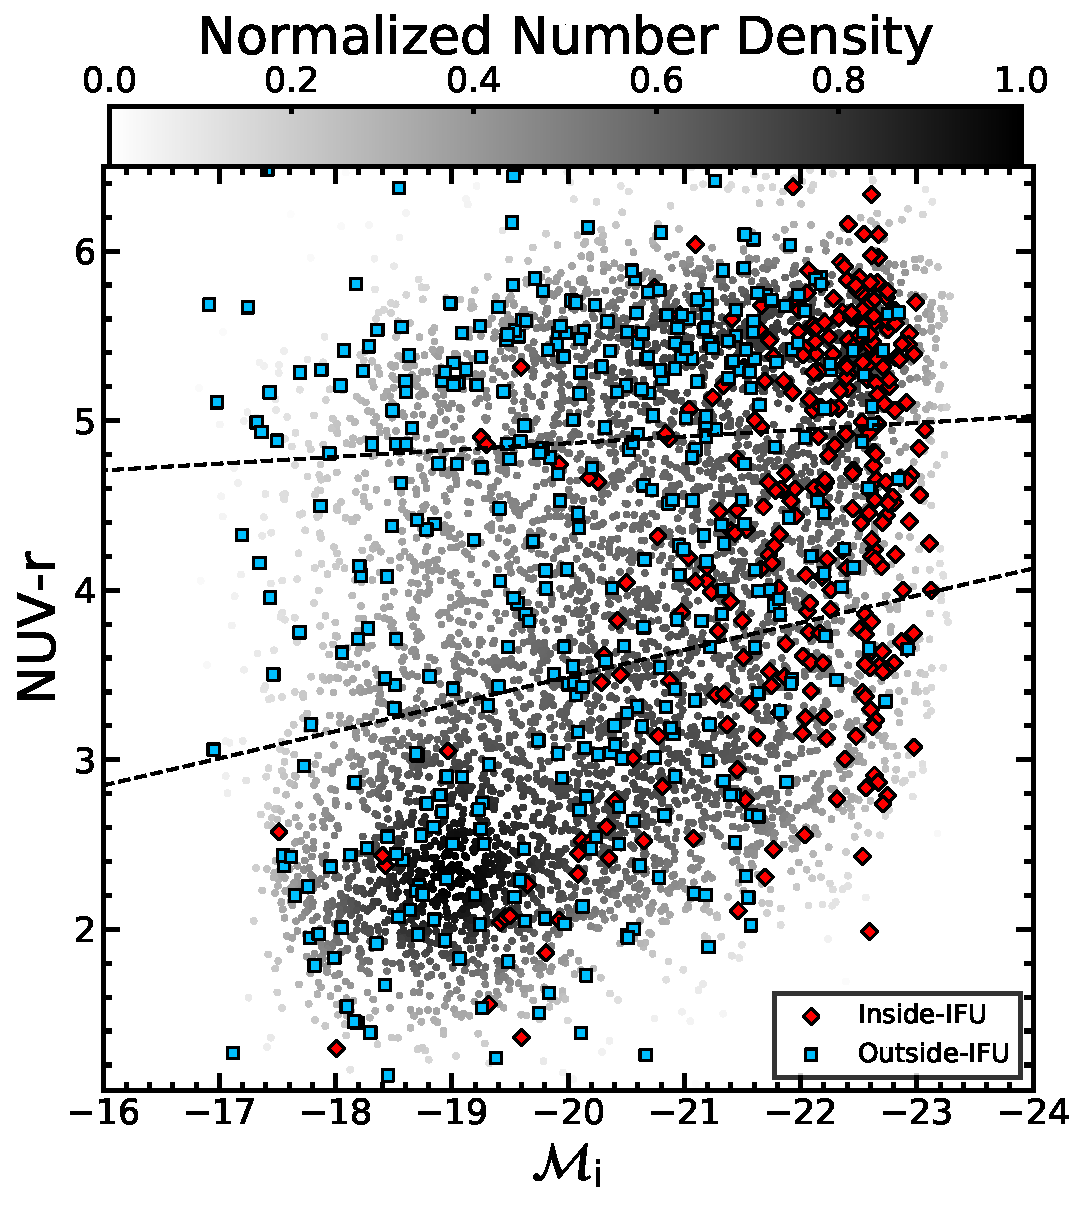
\includegraphics[width=3in]{fig/color-mag.pdf}
\caption[Color-magnitude distribution of the MaNGA galaxies]{Color-magnitude diagram for MaNGA galaxies ({\it colored circles}). The color of the symbol reflects the local density around each data point in this color-magnitude plane, as indicated by the color bar on the top. The MaNGA galaxies with close companions are marked with {\it grey diamonds}. From top to bottom, the dashed lines divide the sample into red sequence, green valley, and blue cloud. The star-forming galaxy sample used in this paper are the galaxies below the lower dividing line.}
\label{fig:CMD}
\end{figure}
%%%%%%%%%%%%%%%%%%%%%%%%%%%%%%%%%%%%%%%%%%%%%%

%%%%%%%%%%%%%%%%%%%%%%%%%%%%%%%%%%%%%%%%%%%%%%
\begin{figure}
\centering
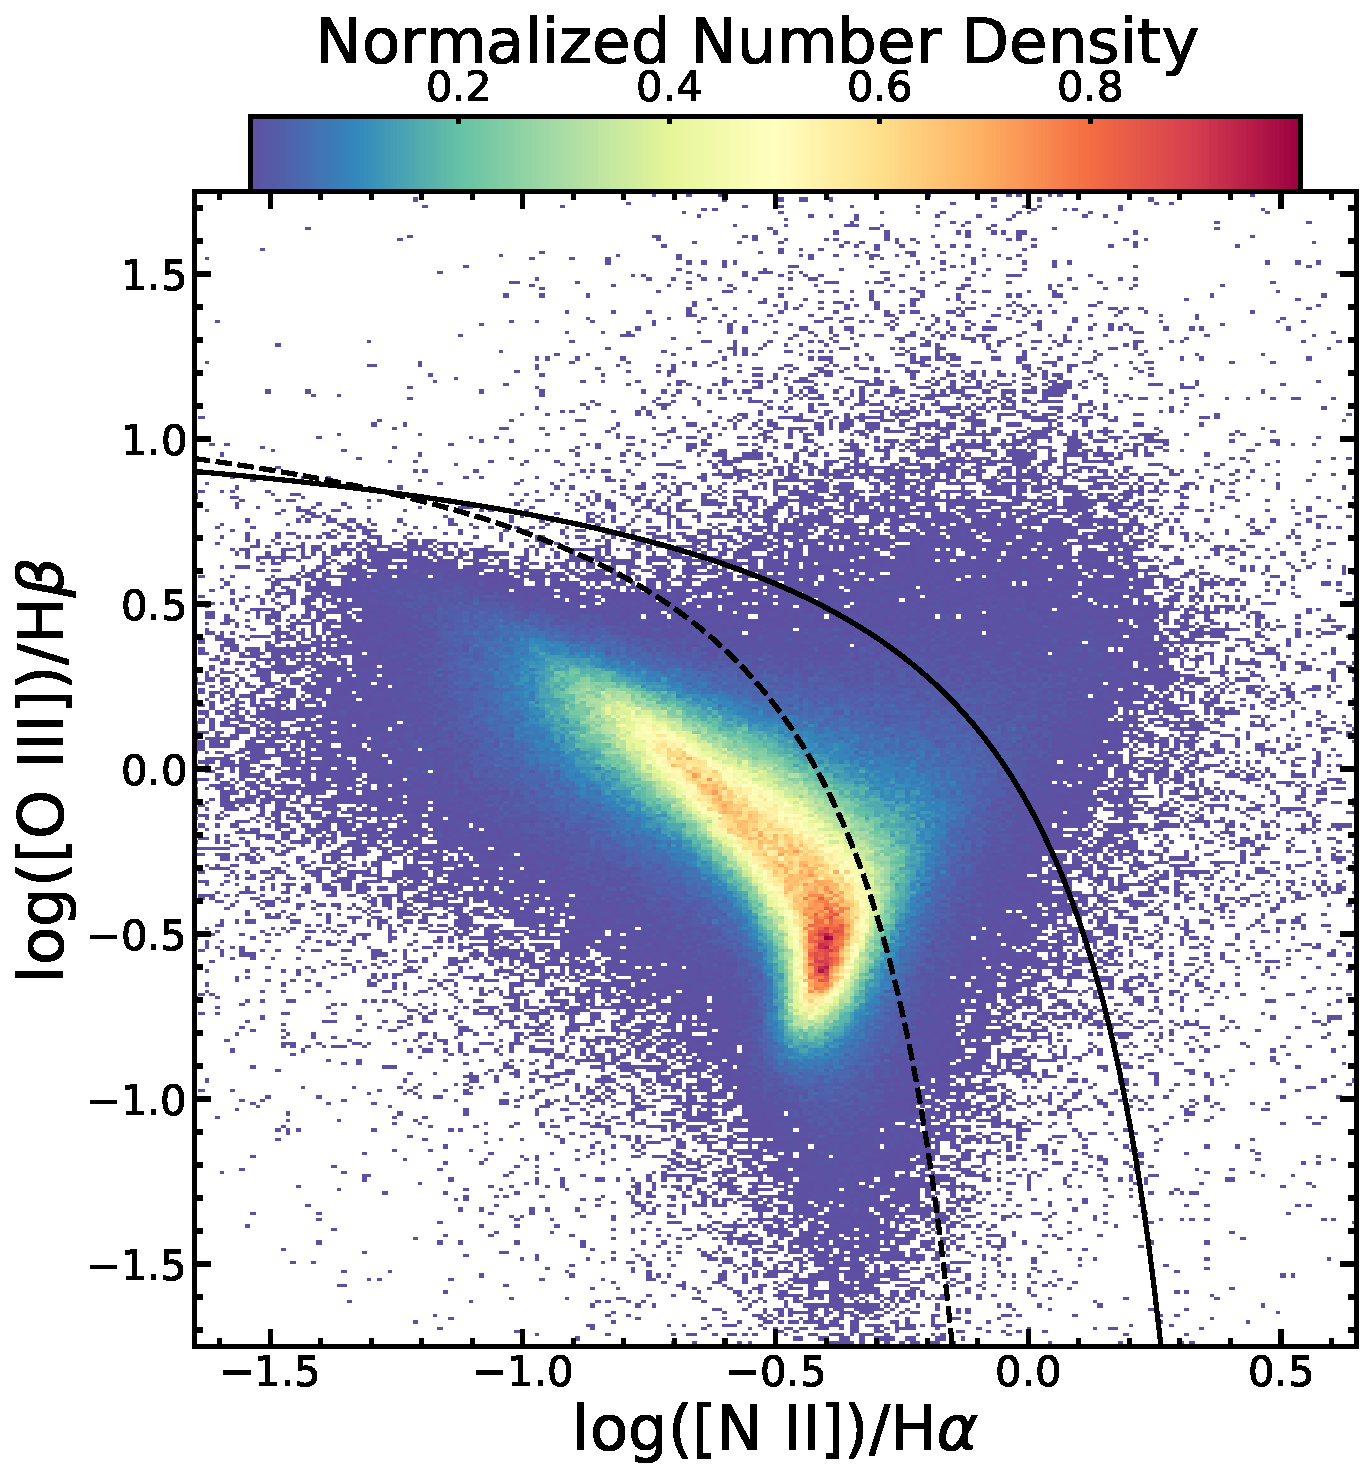
\includegraphics[width=3in]{fig/bpt_spax.pdf}
\caption[BPT classification of MaNGA spaxels.]{The 2-D histogram showing the BPT classification \citep{Baldwin:1981} of individual spaxels within our star-forming control and pair samples. The color of each bin represents the number density of spaxels, normalized to one. The black line represents the theoretically determined maximum starburst line of \citet{Kewley:2001}. This shows the capability of the CMD to select star-forming galaxies as most of the spaxels within the selected galaxies fall beneath the starburst line.}
\label{fig:bpt_spax}
\end{figure}
%%%%%%%%%%%%%%%%%%%%%%%%%%%%%%%%%%%%%%%%%%%%%%

%%%%%%%%%%%%%%%%%%%%%%%%%%%%%%%%%%%%%%%%%%%%%%
\begin{figure}
\centering
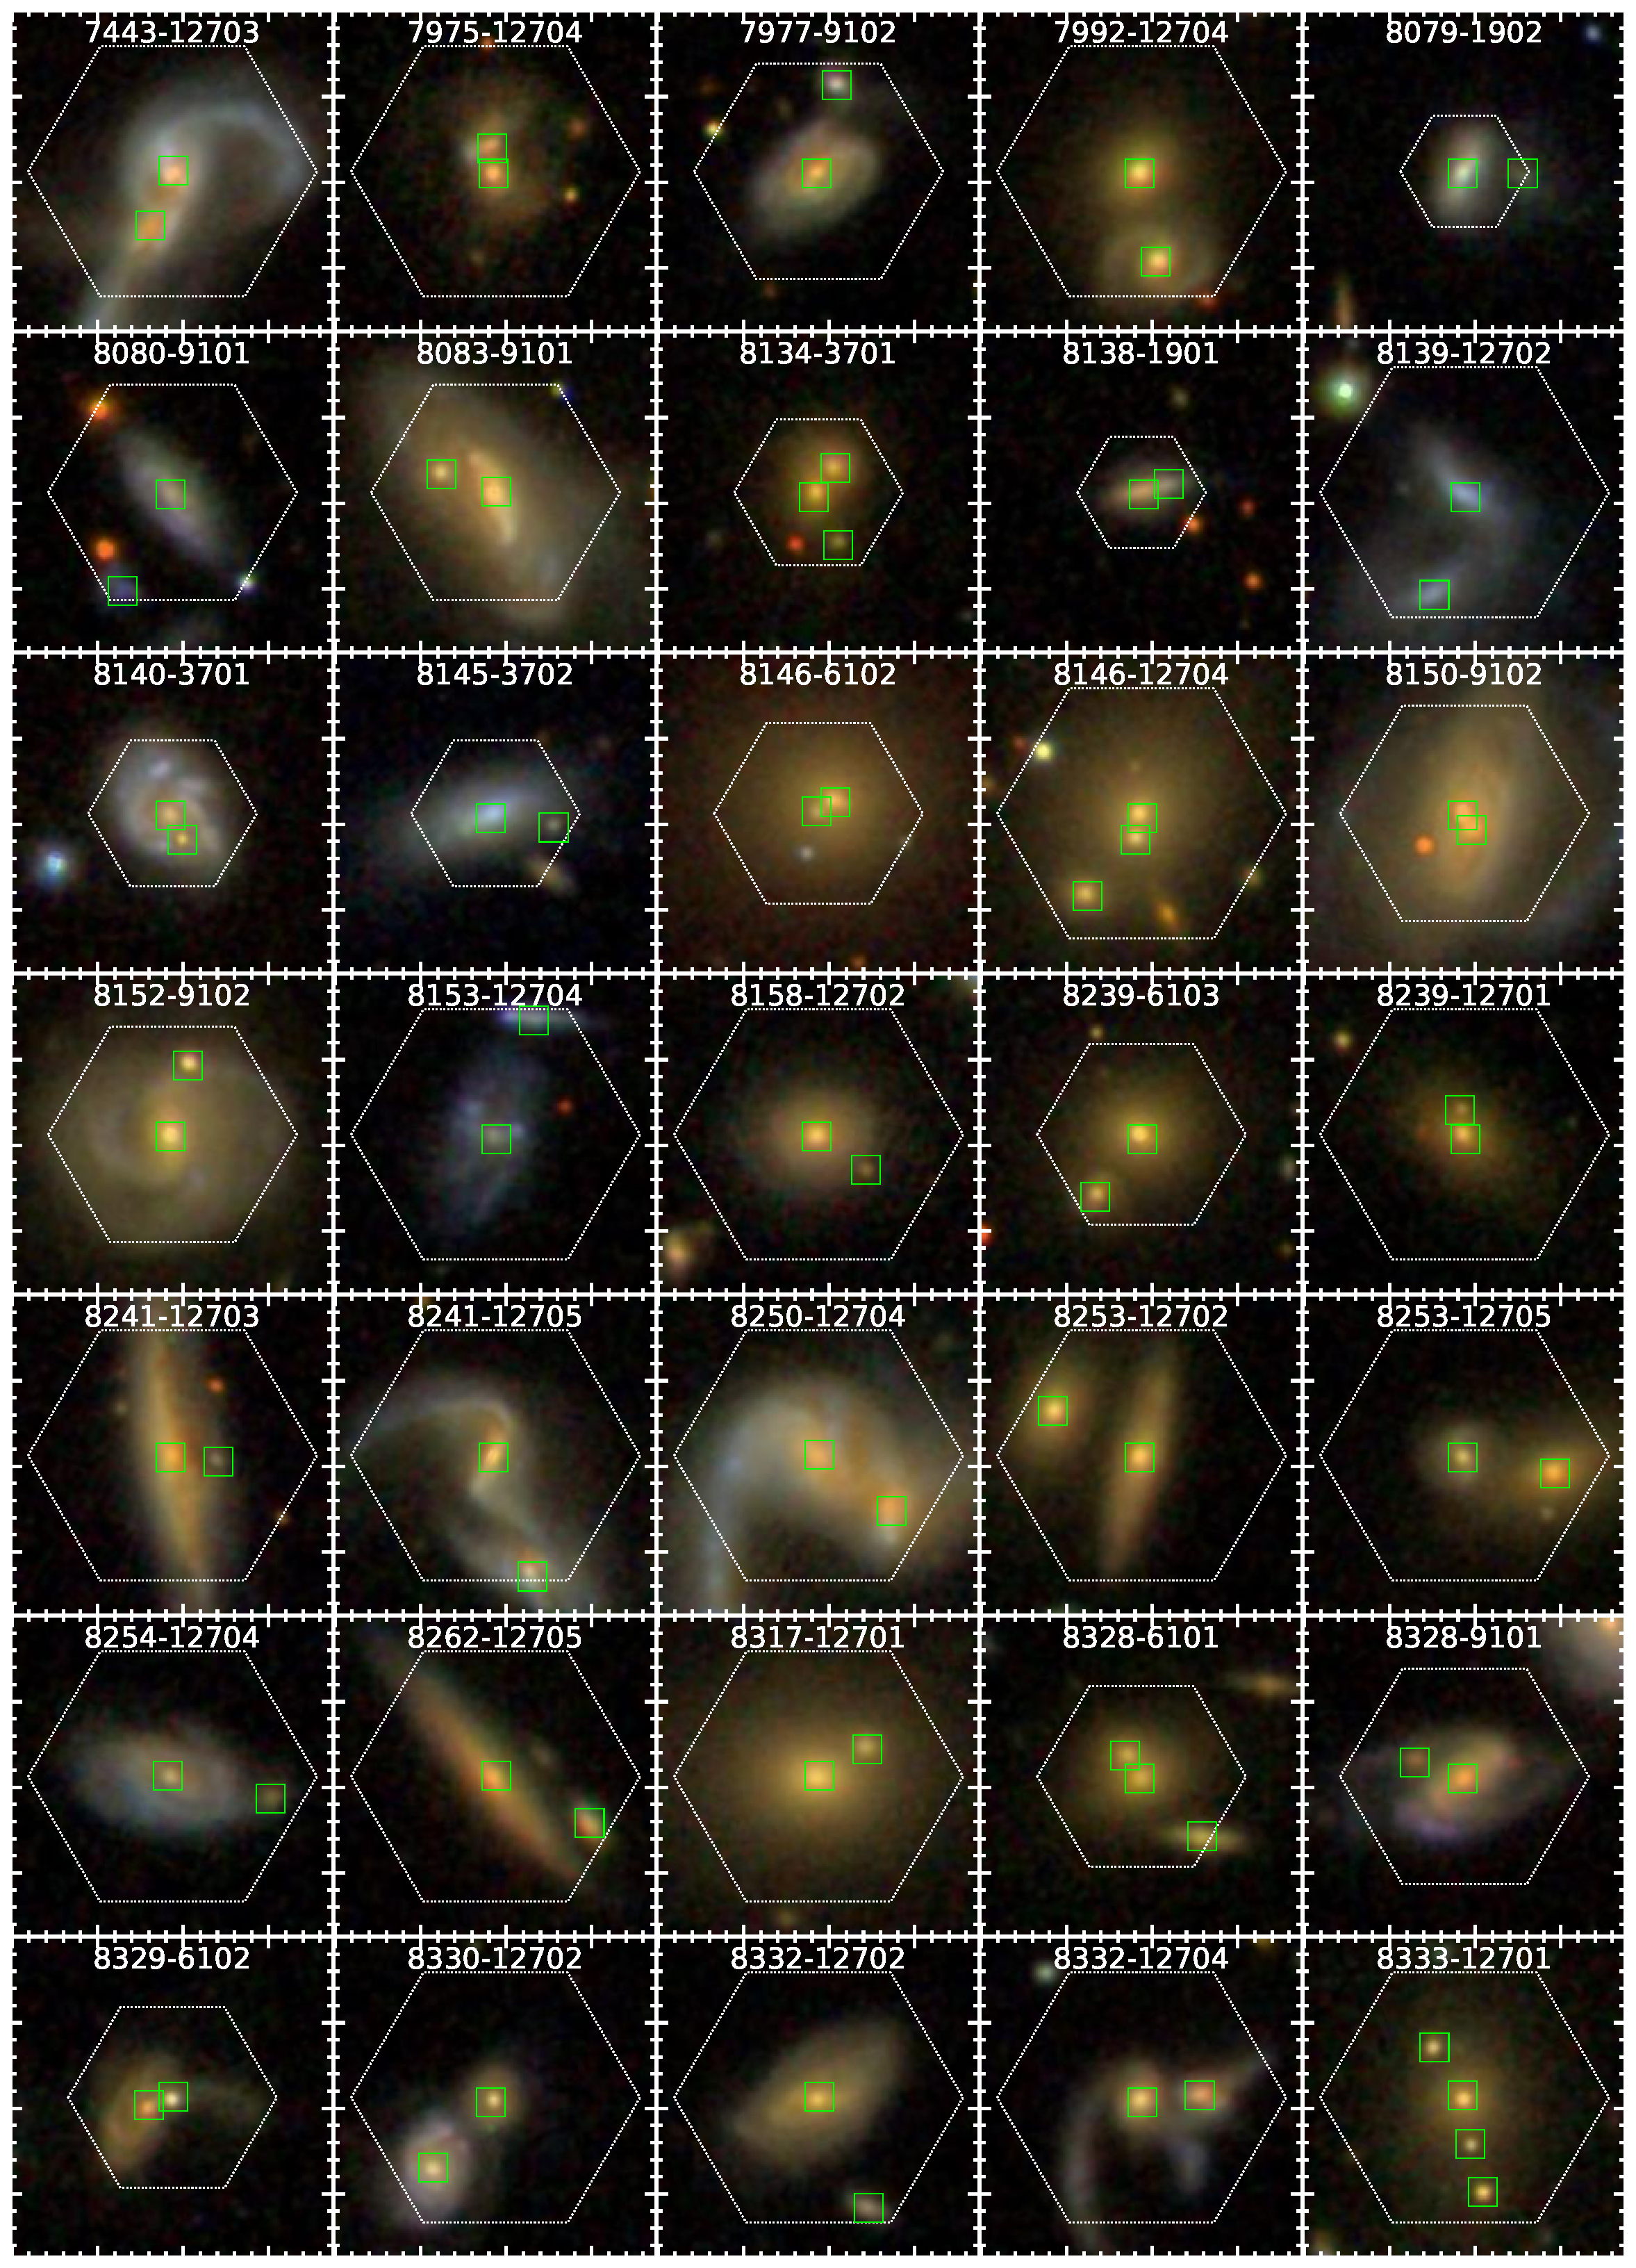
\includegraphics[width=\linewidth]{fig/pair_collage.pdf}
\caption[A collage of a subset of the inside-IFU pairs.]{A collage of a subset of the inside-IFU pairs. Each panel contains a 40$^{\arcsec}$ cutout of the SDSS pseudocolor image for the galaxy pair. The minor ticks on each panel's axis represents 2$^{\arcsec}$. The green squares highlight the identified galaxy pairs. }
\label{fig:collage}
\end{figure}
%%%%%%%%%%%%%%%%%%%%%%%%%%%%%%%%%%%%%%%%%%%%%%

%%%%%%%%%%%%%%%%%%%%%%%%%%%%%%%%%%%%%%%%%%%%%%
\begin{figure*}
\centering
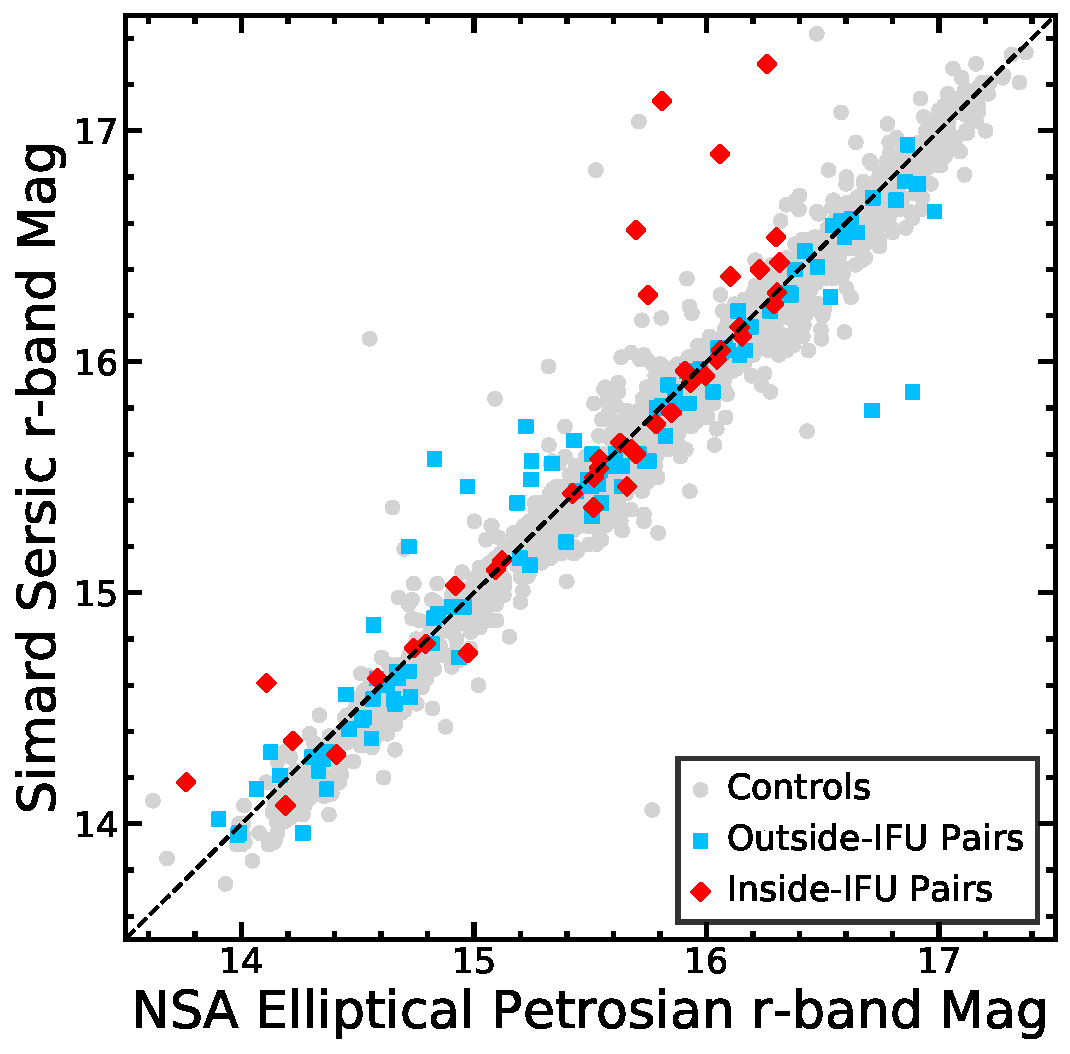
\includegraphics[width=3in]{fig/mag_comp.pdf}
\caption[The comparison between the r-band magnitudes in Simard+11 and NSA catalog]{The comparison between the S\'ersic r-band apparent magnitude in \citet{Simard:2011} and the Elliptical Petrosian r-band apparent magnitude. The grey circles represent galaxies in the control sample, the blue squares represent galaxies in the outside-IFU sample, and the red diamonds represent the galaxies in the inside-IFU sample. Regardless of the sample, all of the galaxies covered by both of the catalogs have a similar apparent magnitude calculated from either sample.}
\label{fig:mag_comp}
\end{figure*}
%%%%%%%%%%%%%%%%%%%%%%%%%%%%%%%%%%%%%%%%%%%%%%

%%%%%%%%%%%%%%%%%%%%%%%%%%%%%%%%%%%%%%%%%%%%%%
\begin{figure*}
\centering
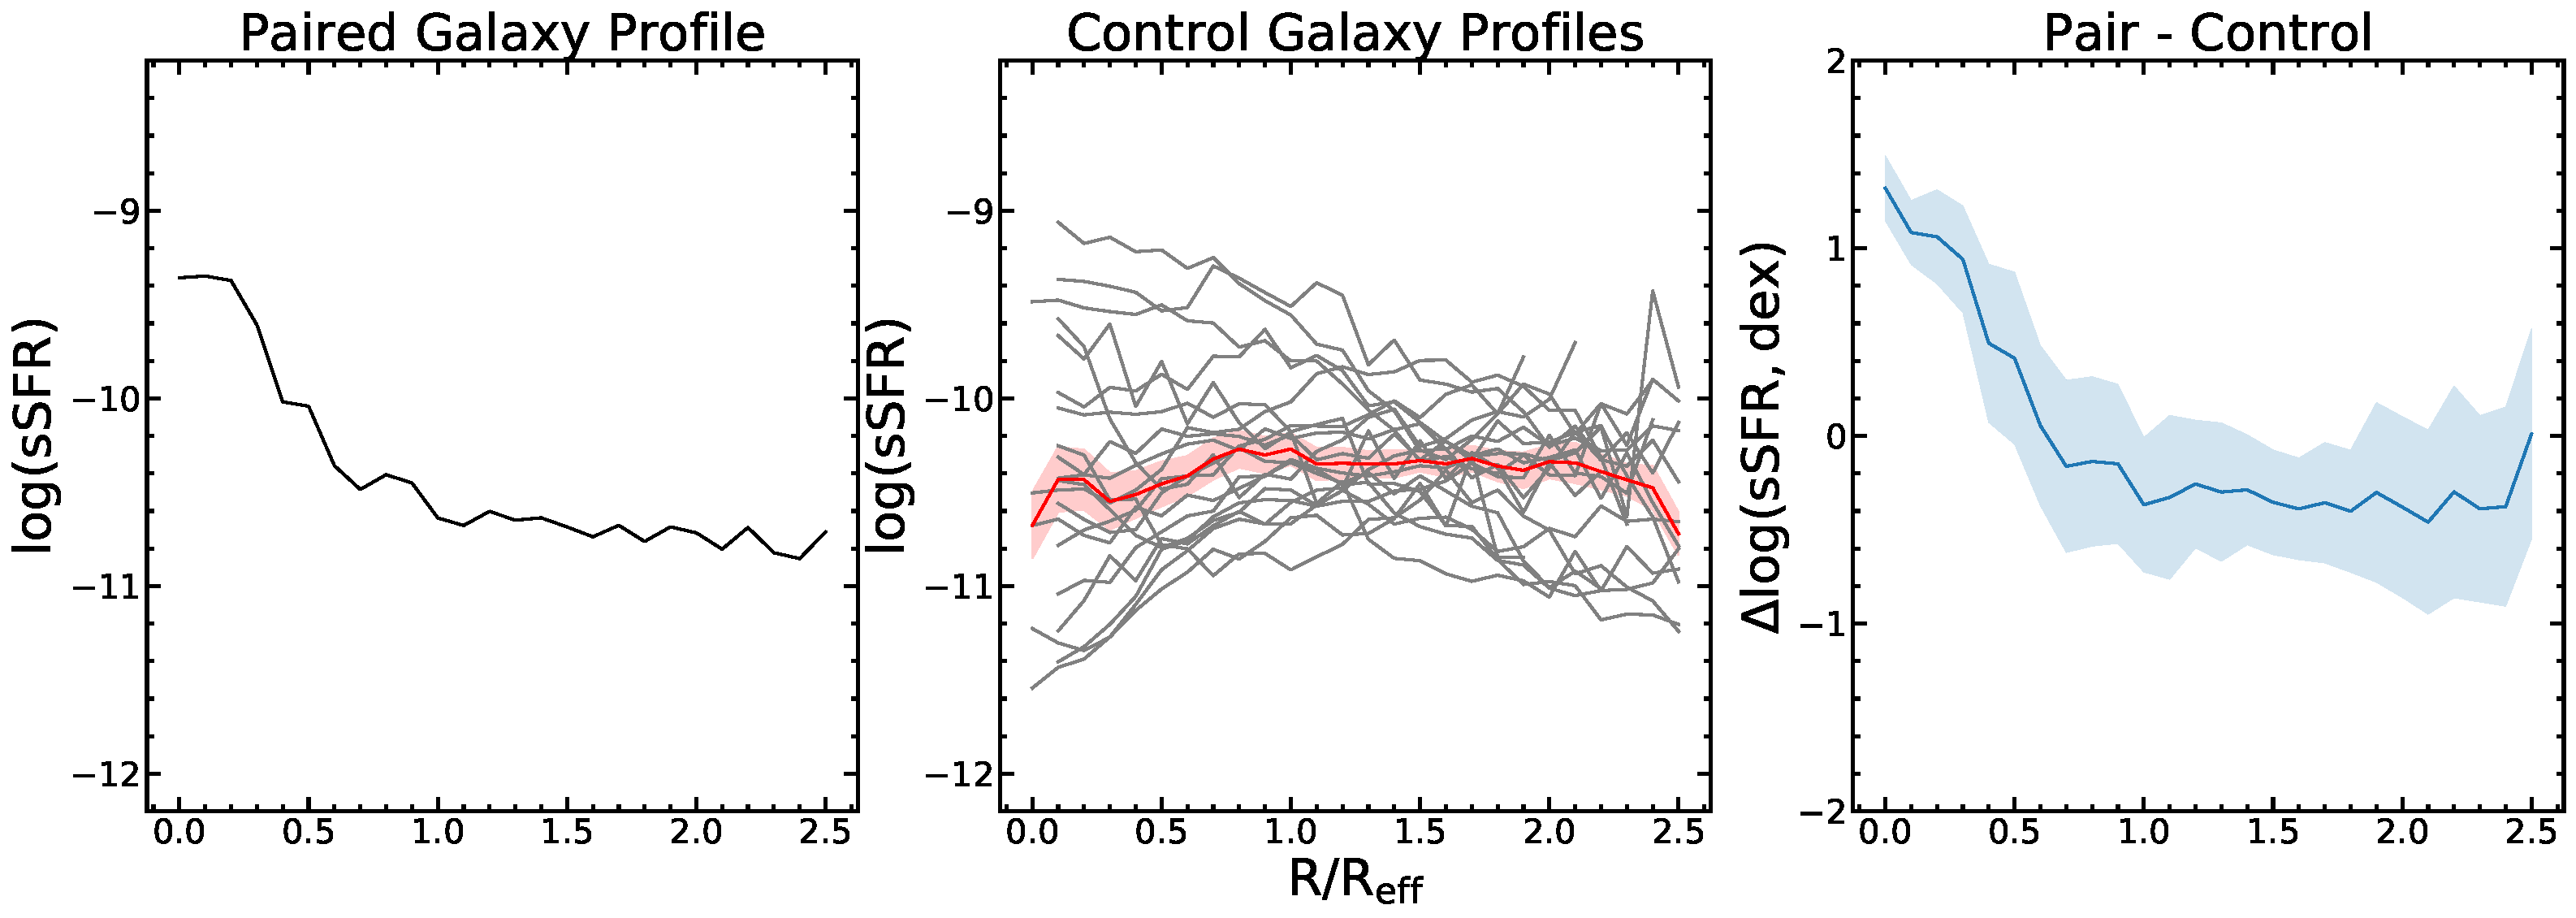
\includegraphics[width=\linewidth]{fig/8083-12703.pdf}
\caption[Example of the difference profiles for the mass-redshift selected control sample.]{The process for building the tailored control sample. The Left panel shows the paired galaxy's profile for sSFR. The Middle panel shows the profiles for sSFR for the selected 20 control galaxies in gray. The red profile is the median profile of the 20 control galaxies where the highlighted region about the profile is the standard error of the mean. The Right panel shows the difference between pair's profile and the stacked control profile.}
\label{fig:dex}
\end{figure*}
%%%%%%%%%%%%%%%%%%%%%%%%%%%%%%%%%%%%%%%%%%%%%%

%%%%%%%%%%%%%%%%%%%%%%%%%%%%%%%%%%%%%%%%%%%%%%
\begin{figure*}
\centering
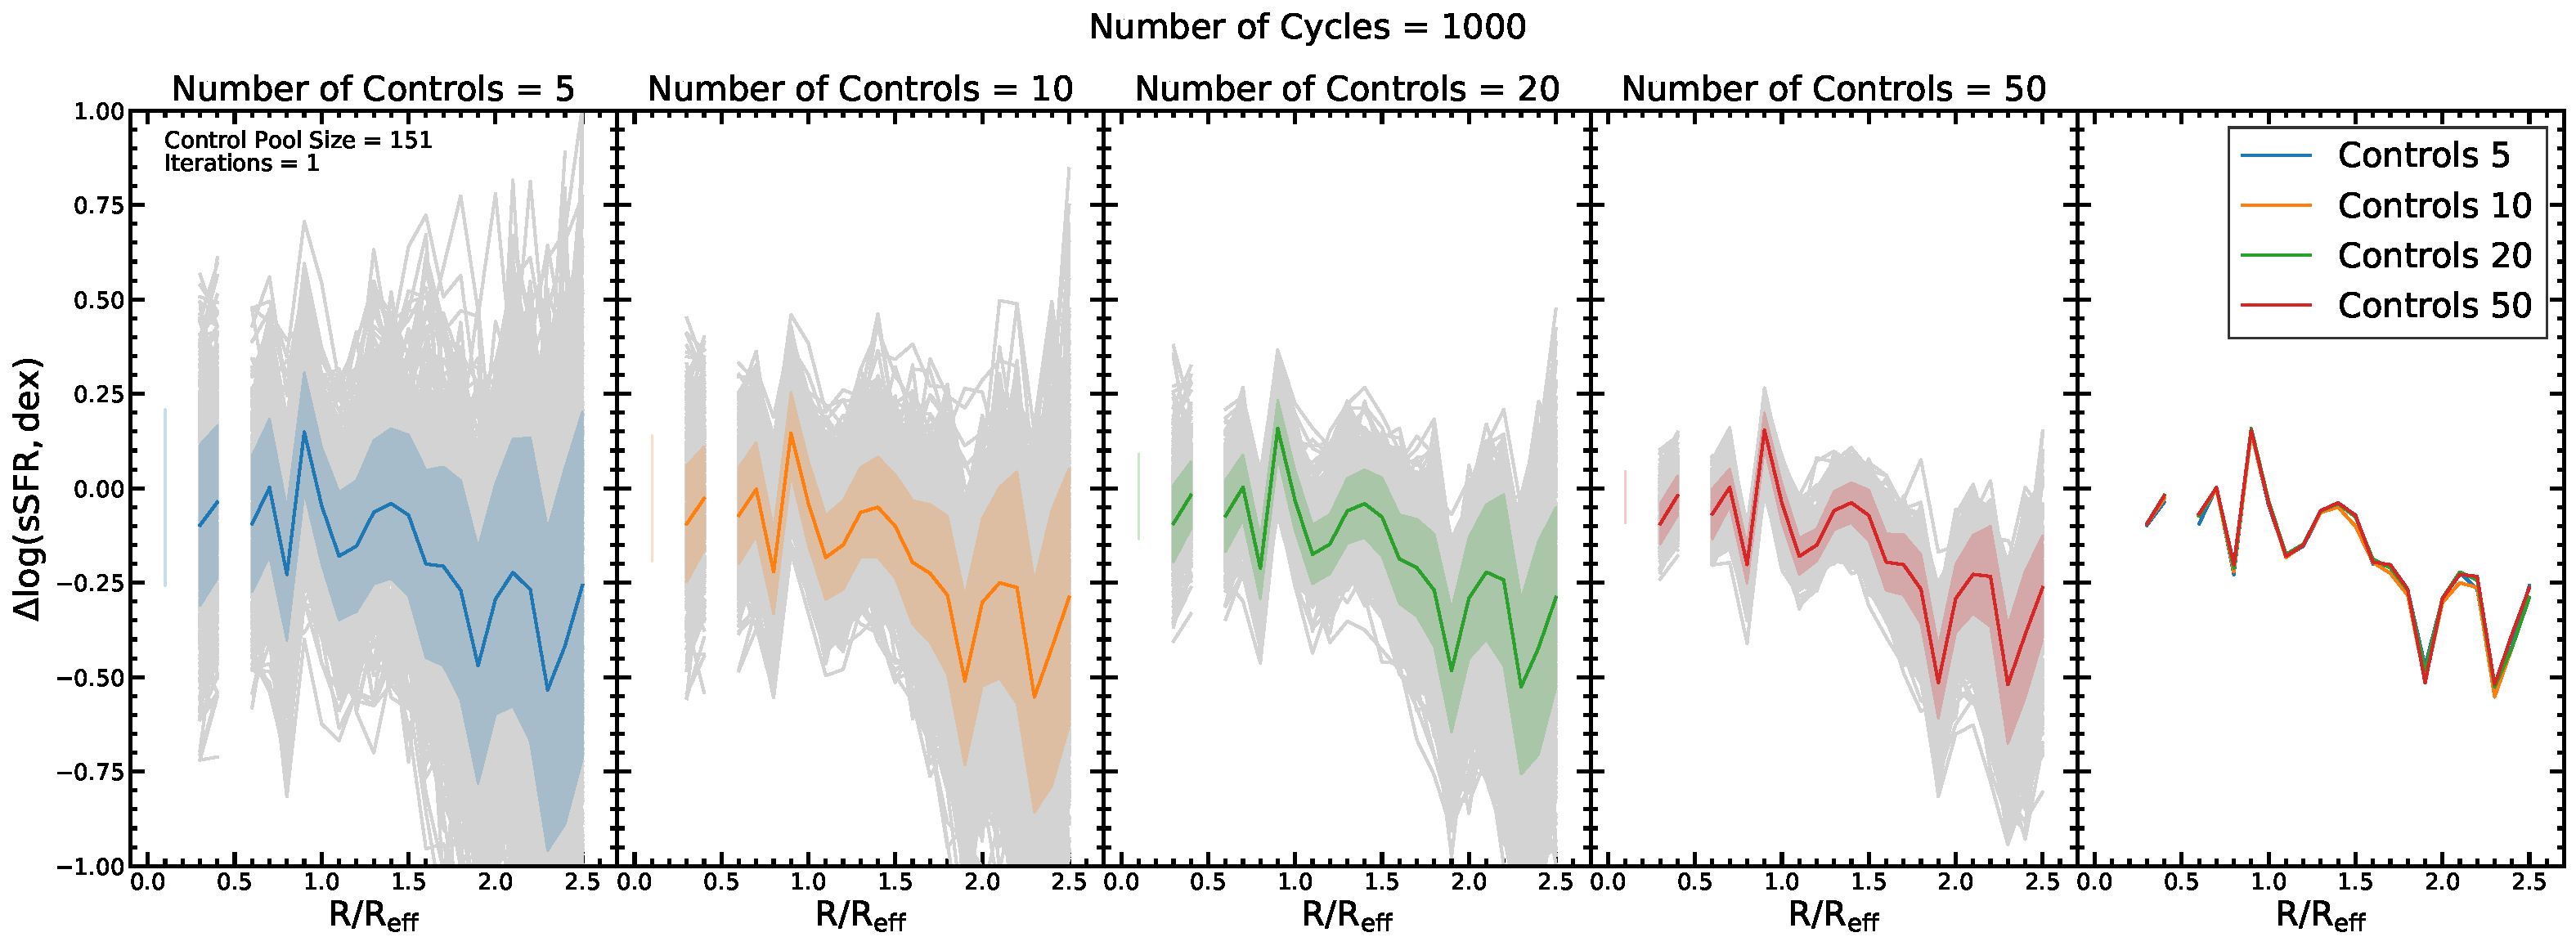
\includegraphics[width=\linewidth]{fig/8485-3704.pdf}
\caption[Example of bootstrapping to quantify the deviation of the random subsample of controls]{An example of the bootstrapping used to quantify the errors associated with the random selection of the control subsample. From left to right, the first four panels show the individual dex profiles after a random sub-selection in grey. The random sub-selection is run 1000 times and the median profile after the 1000 cycles is given by the colored profile. The highlighted region about the colored profiles is the standard error of the mean of the median profile. From left to right each panel shows the random selection for a different number of controls to select; 5, 10, 20, and 50 controls. The panel on the right end shows the median profiles of all of the preceding panels. }
\label{fig:bootstrap}
\end{figure*}
%%%%%%%%%%%%%%%%%%%%%%%%%%%%%%%%%%%%%%%%%%%%%%

%%%%%%%%%%%%%%%%%%%%%%%%%%%%%%%%%%%%%%%%%%%%%%
\begin{figure}
\centering
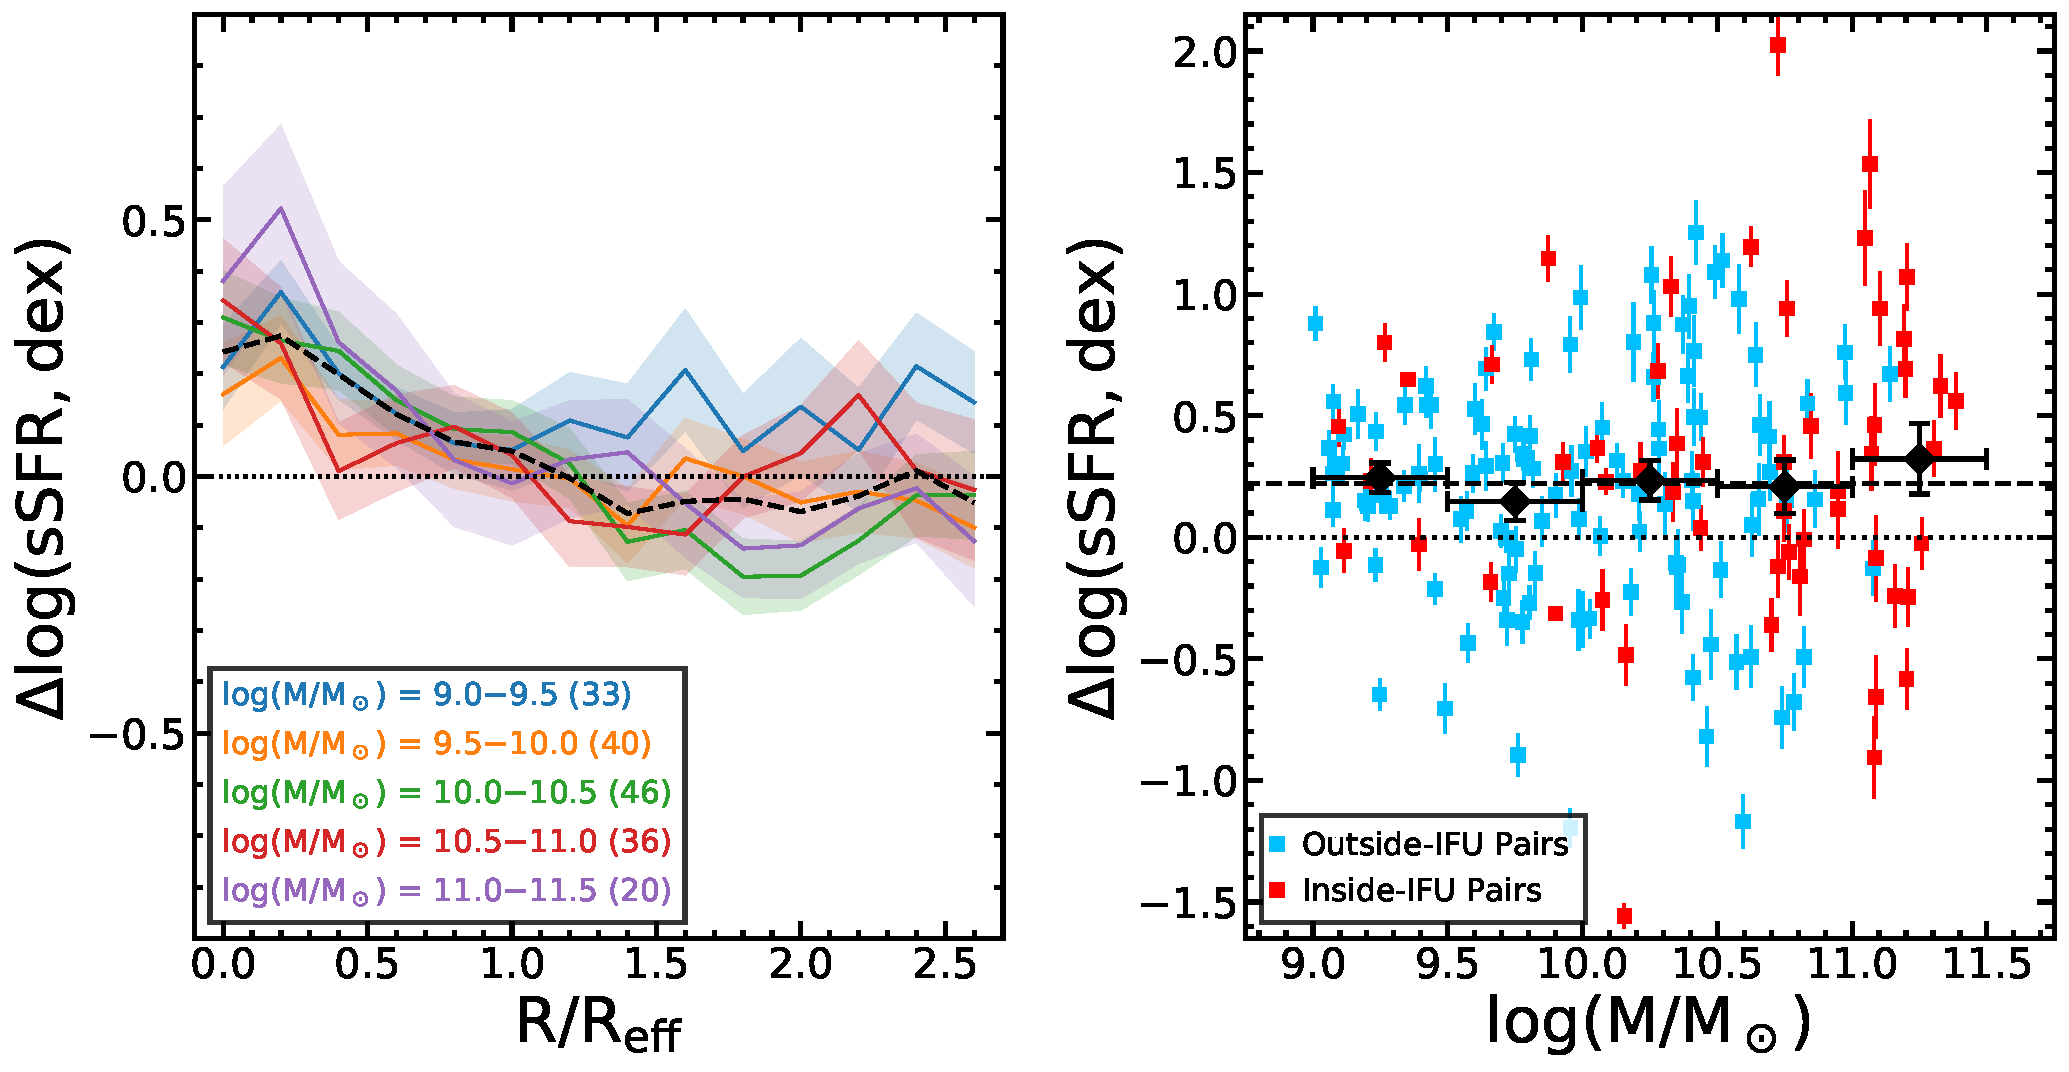
\includegraphics[width=\linewidth]{fig/ssfr_mass.pdf}
\caption[The $\Delta$log(sSFR) split by stellar mass.]{The $\Delta$log(sSFR) split into separate stellar mass bins. The left column gives the stacked difference profiles. The highlighted region about the profiles represents the standard error of the mean of the profile. The right column gives the nuclear $\Delta$log(sSFR) values. The black squares are the mean values within a stellar mass bin (where the size of the bins are shown the the horizontal error bars). The vertical error bars on the black squares represent the standard deviation within the bin. The top row is the inside-IFU sample, the middle row is the outside-IFU sample, and the bottom row is the combination of the two samples.}
\label{fig:ssfr_mass}
\end{figure}
%%%%%%%%%%%%%%%%%%%%%%%%%%%%%%%%%%%%%%%%%%%%%%

%%%%%%%%%%%%%%%%%%%%%%%%%%%%%%%%%%%%%%%%%%%%%%
\begin{figure}
\centering
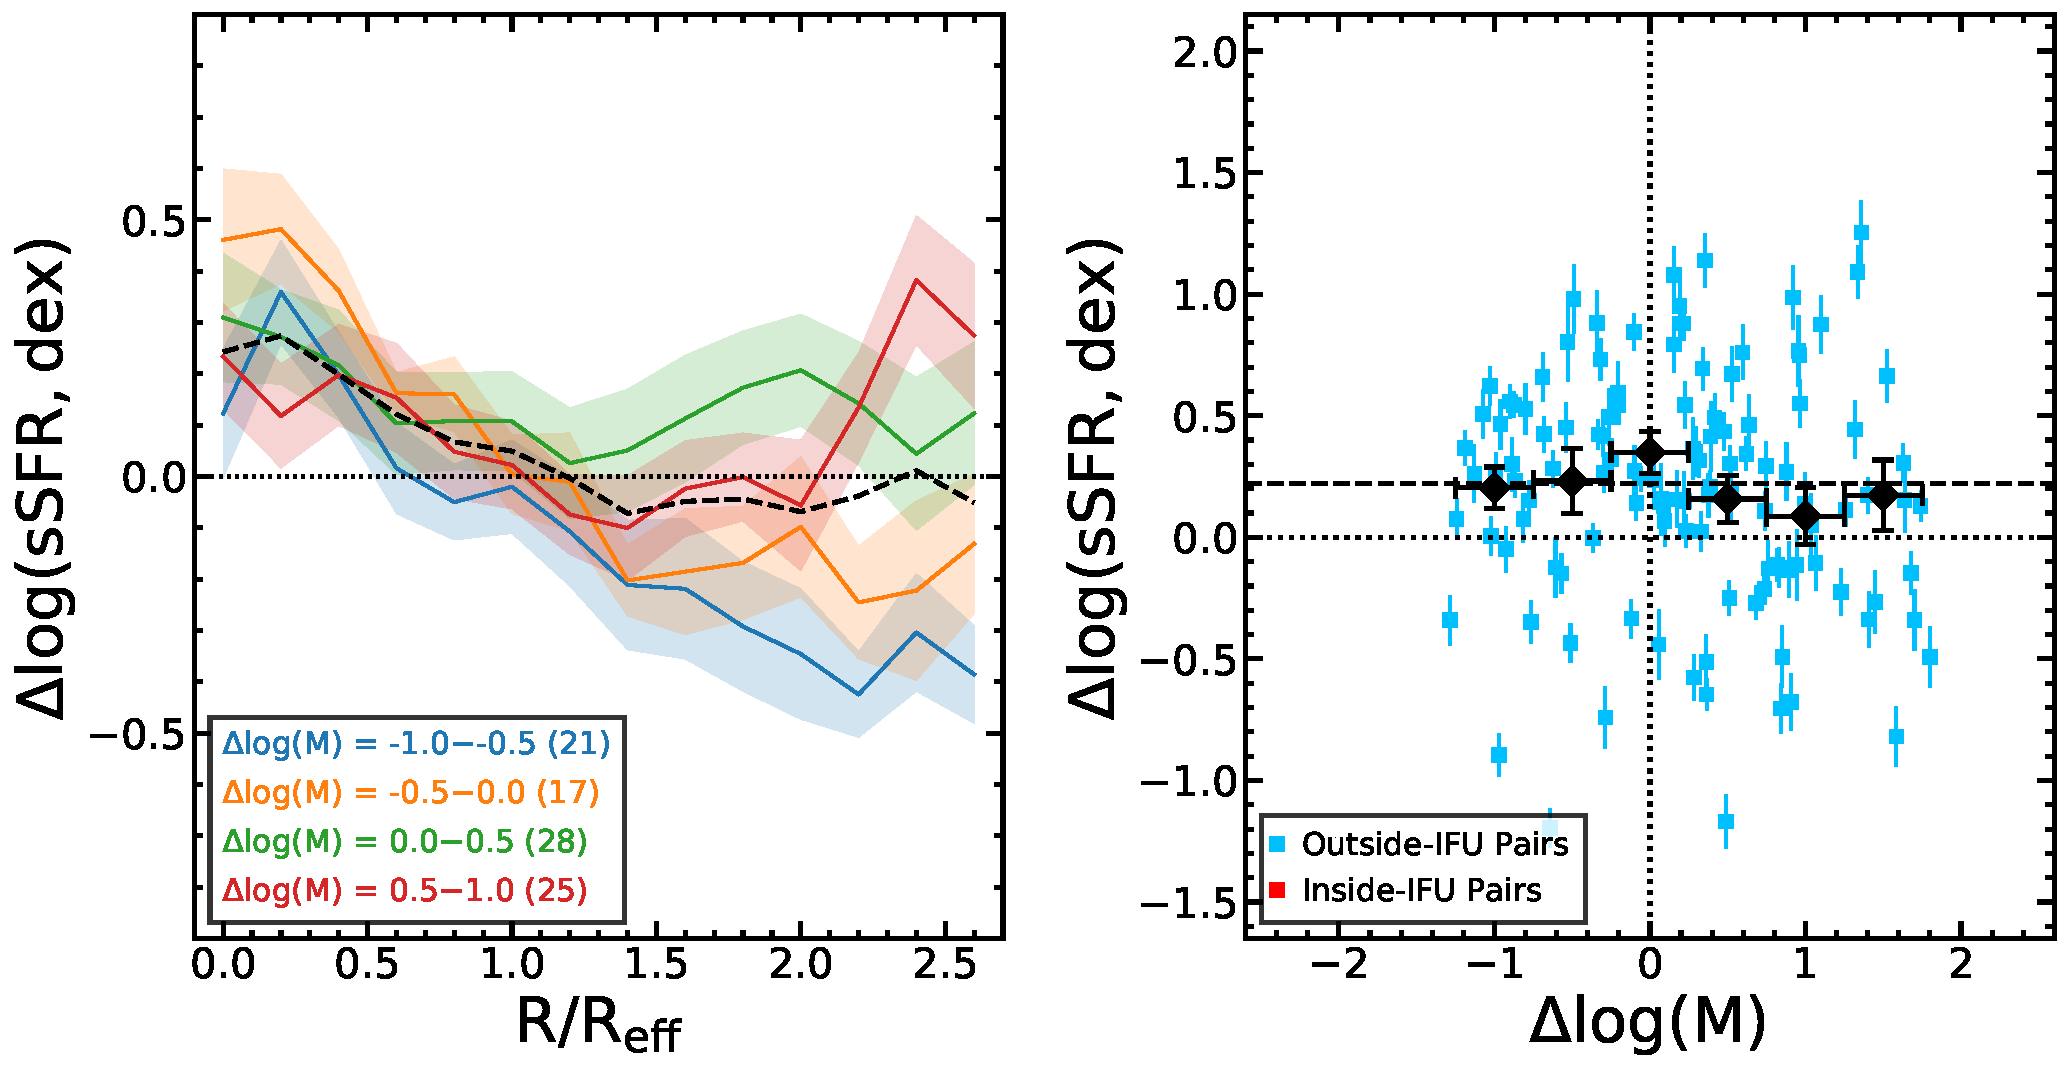
\includegraphics[width=\linewidth]{fig/ssfr_dm.pdf}
\caption[The $\Delta$log(sSFR) split by mass ratio.]{Same as Figure \ref{fig:ssfr_mass} but split into separate mass ratio bins.}
\label{fig:ssfr_dm}
\end{figure}
%%%%%%%%%%%%%%%%%%%%%%%%%%%%%%%%%%%%%%%%%%%%%%

%%%%%%%%%%%%%%%%%%%%%%%%%%%%%%%%%%%%%%%%%%%%%%
\begin{figure}
\centering
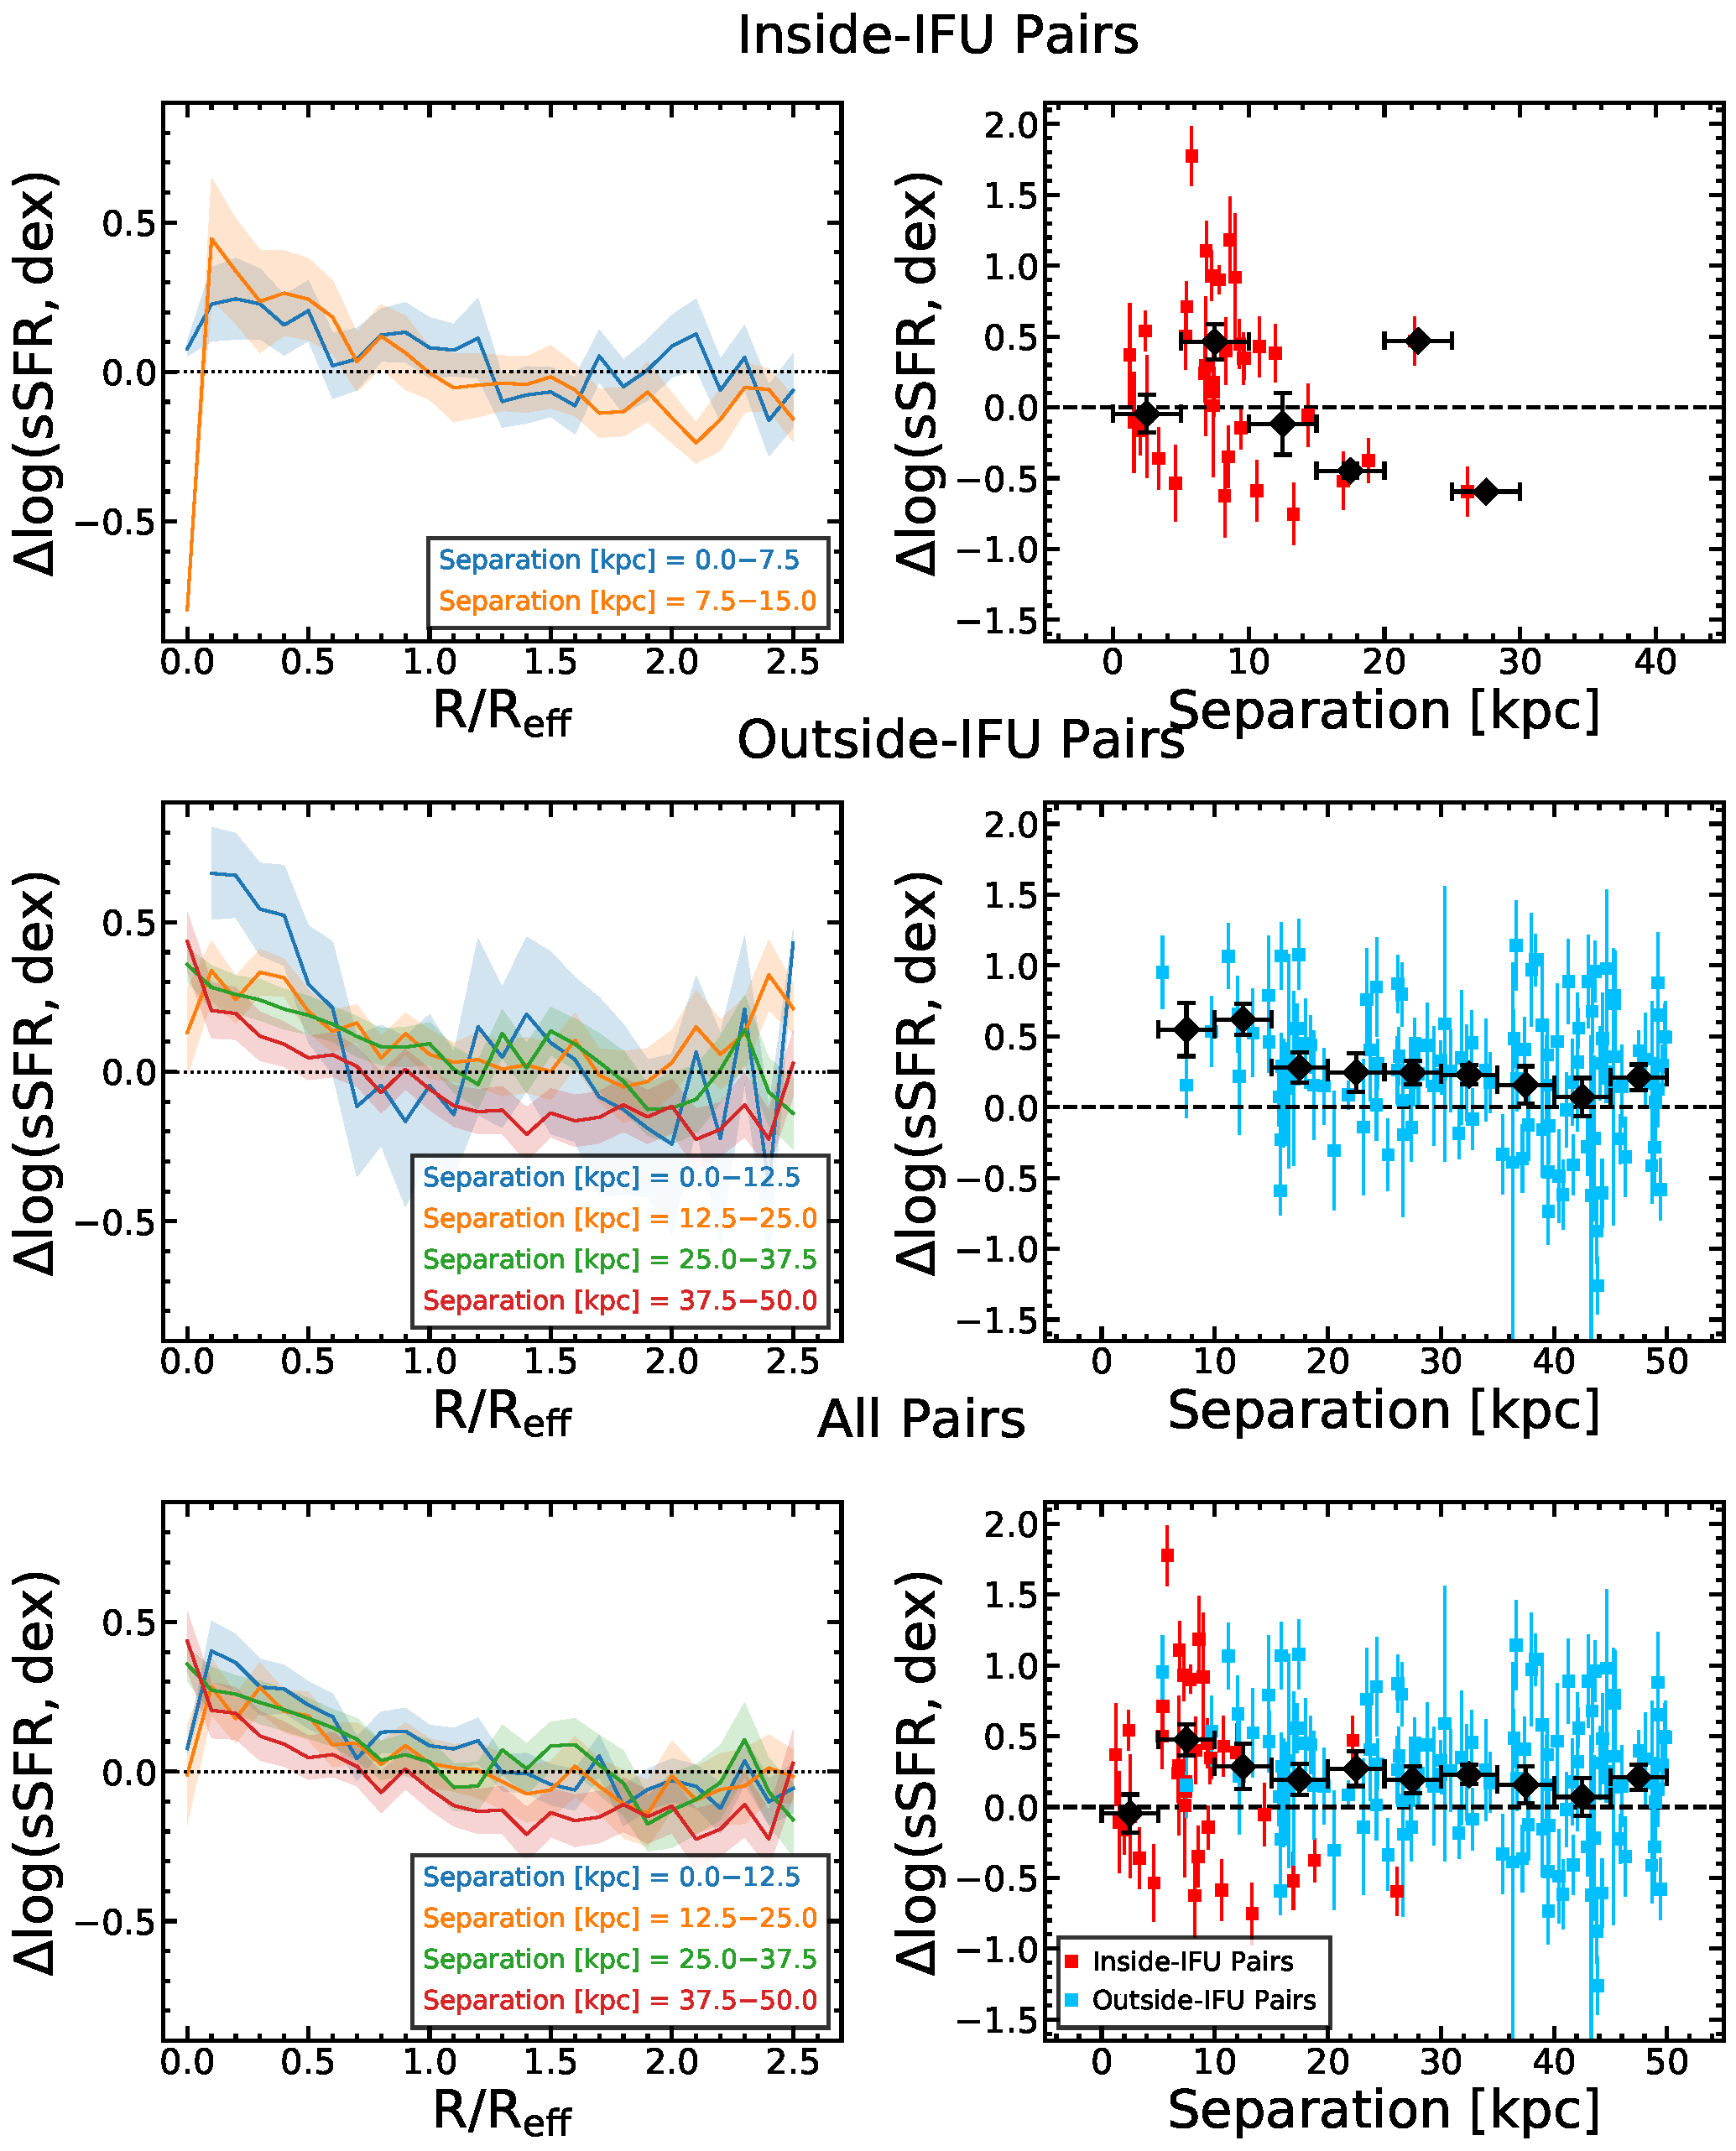
\includegraphics[width=\linewidth]{fig/ssfr_sep.pdf}
\caption[The $\Delta$log(sSFR) split by projected separation.]{Same as Figure \ref{fig:ssfr_mass} but split into separate projected separation bins.}
\label{fig:ssfr_sep}
\end{figure}
%%%%%%%%%%%%%%%%%%%%%%%%%%%%%%%%%%%%%%%%%%%%%%

%%%%%%%%%%%%%%%%%%%%%%%%%%%%%%%%%%%%%%%%%%%%%%
\begin{figure}
\centering
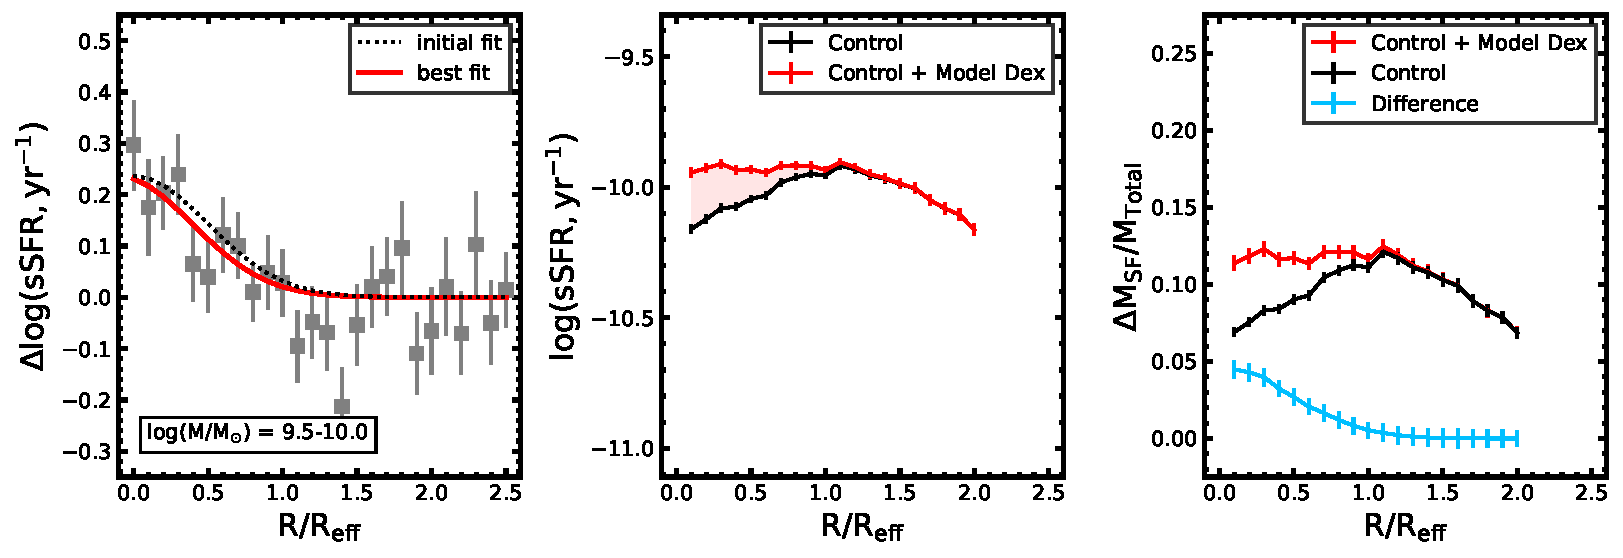
\includegraphics[width=\linewidth]{fig/mass_gain_1.pdf}
\caption[Example of the calculation of the fractional mass gain due to merger induced star formation for a single mass bin.]{In the Left panel we fit a model gaussian to the $\Delta$log(sSFR) profiles. In the Middle panel we plot the log(sSFR) profile for the stacked profiles of the control galaxies (black). We then add the modeled $\Delta$log(sSFR) profile to the control profile (red). The error bars represent the standard error of the mean of the profiles. In the Right panel we show the fractional mass gain due to star formation in the control galaxies (black) and in the paired galaxies (red). The blue profile is the subtraction between the pairs and controls and represents the fractional mass gain due to merger induced star formation. The error bars represent the standard error of the mean of the profiles. }
\label{fig:mass_gain}
\end{figure}
%%%%%%%%%%%%%%%%%%%%%%%%%%%%%%%%%%%%%%%%%%%%%%

%%%%%%%%%%%%%%%%%%%%%%%%%%%%%%%%%%%%%%%%%%%%%%
\begin{figure}
\centering
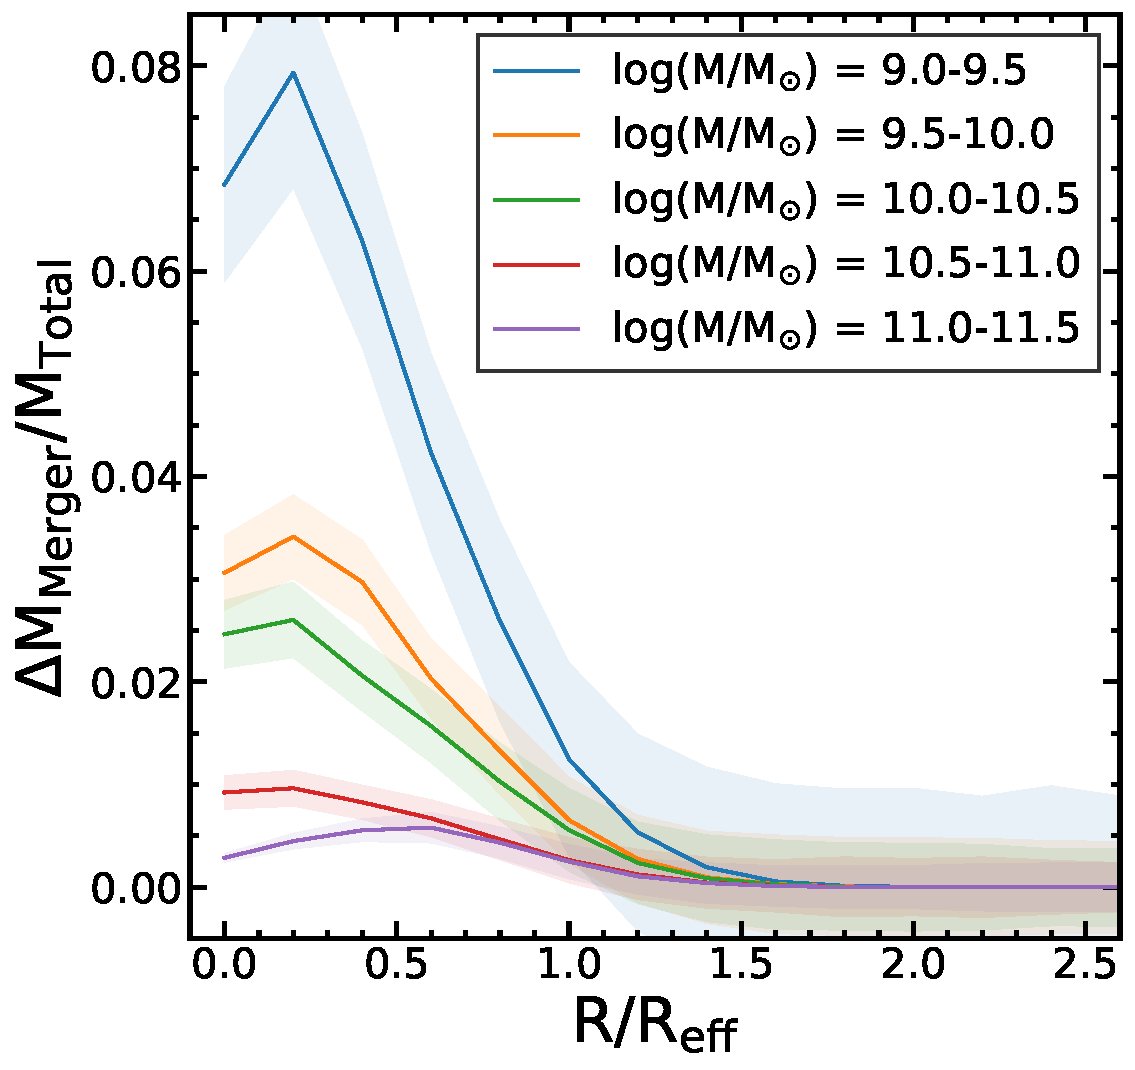
\includegraphics[width=3in]{fig/mass_gain.pdf}
\caption[The fractional mass gain due to merger induced star formation.]{The fractional mass gain due to merger induced star formation over a dynamical timescale, $\tau$ $=$ 1 Gyr. The highlighted region represents the propagated standard errors of the mean of the stacked log(sSFR) profiles. }
\label{fig:mass_gain_sum}
\end{figure}
%%%%%%%%%%%%%%%%%%%%%%%%%%%%%%%%%%%%%%%%%%%%%%

\end{document}